% Options for packages loaded elsewhere
\PassOptionsToPackage{unicode}{hyperref}
\PassOptionsToPackage{hyphens}{url}
%
\documentclass[
]{article}
\usepackage{lmodern}
\usepackage{amssymb,amsmath}
\usepackage{ifxetex,ifluatex}
\ifnum 0\ifxetex 1\fi\ifluatex 1\fi=0 % if pdftex
  \usepackage[T1]{fontenc}
  \usepackage[utf8]{inputenc}
  \usepackage{textcomp} % provide euro and other symbols
\else % if luatex or xetex
  \usepackage{unicode-math}
  \defaultfontfeatures{Scale=MatchLowercase}
  \defaultfontfeatures[\rmfamily]{Ligatures=TeX,Scale=1}
\fi
% Use upquote if available, for straight quotes in verbatim environments
\IfFileExists{upquote.sty}{\usepackage{upquote}}{}
\IfFileExists{microtype.sty}{% use microtype if available
  \usepackage[]{microtype}
  \UseMicrotypeSet[protrusion]{basicmath} % disable protrusion for tt fonts
}{}
\makeatletter
\@ifundefined{KOMAClassName}{% if non-KOMA class
  \IfFileExists{parskip.sty}{%
    \usepackage{parskip}
  }{% else
    \setlength{\parindent}{0pt}
    \setlength{\parskip}{6pt plus 2pt minus 1pt}}
}{% if KOMA class
  \KOMAoptions{parskip=half}}
\makeatother
\usepackage{xcolor}
\IfFileExists{xurl.sty}{\usepackage{xurl}}{} % add URL line breaks if available
\IfFileExists{bookmark.sty}{\usepackage{bookmark}}{\usepackage{hyperref}}
\hypersetup{
  pdftitle={Modeling Customer Lifetime and Churn PreventionC},
  hidelinks,
  pdfcreator={LaTeX via pandoc}}
\urlstyle{same} % disable monospaced font for URLs
\usepackage[margin=1in]{geometry}
\usepackage{color}
\usepackage{fancyvrb}
\newcommand{\VerbBar}{|}
\newcommand{\VERB}{\Verb[commandchars=\\\{\}]}
\DefineVerbatimEnvironment{Highlighting}{Verbatim}{commandchars=\\\{\}}
% Add ',fontsize=\small' for more characters per line
\usepackage{framed}
\definecolor{shadecolor}{RGB}{248,248,248}
\newenvironment{Shaded}{\begin{snugshade}}{\end{snugshade}}
\newcommand{\AlertTok}[1]{\textcolor[rgb]{0.94,0.16,0.16}{#1}}
\newcommand{\AnnotationTok}[1]{\textcolor[rgb]{0.56,0.35,0.01}{\textbf{\textit{#1}}}}
\newcommand{\AttributeTok}[1]{\textcolor[rgb]{0.77,0.63,0.00}{#1}}
\newcommand{\BaseNTok}[1]{\textcolor[rgb]{0.00,0.00,0.81}{#1}}
\newcommand{\BuiltInTok}[1]{#1}
\newcommand{\CharTok}[1]{\textcolor[rgb]{0.31,0.60,0.02}{#1}}
\newcommand{\CommentTok}[1]{\textcolor[rgb]{0.56,0.35,0.01}{\textit{#1}}}
\newcommand{\CommentVarTok}[1]{\textcolor[rgb]{0.56,0.35,0.01}{\textbf{\textit{#1}}}}
\newcommand{\ConstantTok}[1]{\textcolor[rgb]{0.00,0.00,0.00}{#1}}
\newcommand{\ControlFlowTok}[1]{\textcolor[rgb]{0.13,0.29,0.53}{\textbf{#1}}}
\newcommand{\DataTypeTok}[1]{\textcolor[rgb]{0.13,0.29,0.53}{#1}}
\newcommand{\DecValTok}[1]{\textcolor[rgb]{0.00,0.00,0.81}{#1}}
\newcommand{\DocumentationTok}[1]{\textcolor[rgb]{0.56,0.35,0.01}{\textbf{\textit{#1}}}}
\newcommand{\ErrorTok}[1]{\textcolor[rgb]{0.64,0.00,0.00}{\textbf{#1}}}
\newcommand{\ExtensionTok}[1]{#1}
\newcommand{\FloatTok}[1]{\textcolor[rgb]{0.00,0.00,0.81}{#1}}
\newcommand{\FunctionTok}[1]{\textcolor[rgb]{0.00,0.00,0.00}{#1}}
\newcommand{\ImportTok}[1]{#1}
\newcommand{\InformationTok}[1]{\textcolor[rgb]{0.56,0.35,0.01}{\textbf{\textit{#1}}}}
\newcommand{\KeywordTok}[1]{\textcolor[rgb]{0.13,0.29,0.53}{\textbf{#1}}}
\newcommand{\NormalTok}[1]{#1}
\newcommand{\OperatorTok}[1]{\textcolor[rgb]{0.81,0.36,0.00}{\textbf{#1}}}
\newcommand{\OtherTok}[1]{\textcolor[rgb]{0.56,0.35,0.01}{#1}}
\newcommand{\PreprocessorTok}[1]{\textcolor[rgb]{0.56,0.35,0.01}{\textit{#1}}}
\newcommand{\RegionMarkerTok}[1]{#1}
\newcommand{\SpecialCharTok}[1]{\textcolor[rgb]{0.00,0.00,0.00}{#1}}
\newcommand{\SpecialStringTok}[1]{\textcolor[rgb]{0.31,0.60,0.02}{#1}}
\newcommand{\StringTok}[1]{\textcolor[rgb]{0.31,0.60,0.02}{#1}}
\newcommand{\VariableTok}[1]{\textcolor[rgb]{0.00,0.00,0.00}{#1}}
\newcommand{\VerbatimStringTok}[1]{\textcolor[rgb]{0.31,0.60,0.02}{#1}}
\newcommand{\WarningTok}[1]{\textcolor[rgb]{0.56,0.35,0.01}{\textbf{\textit{#1}}}}
\usepackage{graphicx,grffile}
\makeatletter
\def\maxwidth{\ifdim\Gin@nat@width>\linewidth\linewidth\else\Gin@nat@width\fi}
\def\maxheight{\ifdim\Gin@nat@height>\textheight\textheight\else\Gin@nat@height\fi}
\makeatother
% Scale images if necessary, so that they will not overflow the page
% margins by default, and it is still possible to overwrite the defaults
% using explicit options in \includegraphics[width, height, ...]{}
\setkeys{Gin}{width=\maxwidth,height=\maxheight,keepaspectratio}
% Set default figure placement to htbp
\makeatletter
\def\fps@figure{htbp}
\makeatother
\setlength{\emergencystretch}{3em} % prevent overfull lines
\providecommand{\tightlist}{%
  \setlength{\itemsep}{0pt}\setlength{\parskip}{0pt}}
\setcounter{secnumdepth}{-\maxdimen} % remove section numbering

\title{Modeling Customer Lifetime and Churn PreventionC}
\author{}
\date{\vspace{-2.5em}}

\begin{document}
\maketitle

\hypertarget{load-required-packages}{%
\subsection{Load required packages}\label{load-required-packages}}

\begin{Shaded}
\begin{Highlighting}[]
\KeywordTok{library}\NormalTok{(dplyr)}
\end{Highlighting}
\end{Shaded}

\begin{verbatim}
## 
## Attaching package: 'dplyr'
\end{verbatim}

\begin{verbatim}
## The following objects are masked from 'package:stats':
## 
##     filter, lag
\end{verbatim}

\begin{verbatim}
## The following objects are masked from 'package:base':
## 
##     intersect, setdiff, setequal, union
\end{verbatim}

\begin{Shaded}
\begin{Highlighting}[]
\KeywordTok{library}\NormalTok{(ggplot2)}
\KeywordTok{library}\NormalTok{(corrplot)}
\end{Highlighting}
\end{Shaded}

\begin{verbatim}
## corrplot 0.84 loaded
\end{verbatim}

\begin{Shaded}
\begin{Highlighting}[]
\KeywordTok{library}\NormalTok{(viridisLite)}
\KeywordTok{library}\NormalTok{(viridis)}
\KeywordTok{library}\NormalTok{(lattice)}
\KeywordTok{library}\NormalTok{(car)}
\end{Highlighting}
\end{Shaded}

\begin{verbatim}
## Loading required package: carData
\end{verbatim}

\begin{verbatim}
## 
## Attaching package: 'car'
\end{verbatim}

\begin{verbatim}
## The following object is masked from 'package:dplyr':
## 
##     recode
\end{verbatim}

\begin{Shaded}
\begin{Highlighting}[]
\KeywordTok{library}\NormalTok{(MASS)}
\end{Highlighting}
\end{Shaded}

\begin{verbatim}
## 
## Attaching package: 'MASS'
\end{verbatim}

\begin{verbatim}
## The following object is masked from 'package:dplyr':
## 
##     select
\end{verbatim}

\begin{Shaded}
\begin{Highlighting}[]
\KeywordTok{library}\NormalTok{(caret)}
\KeywordTok{library}\NormalTok{(pROC)}
\end{Highlighting}
\end{Shaded}

\begin{verbatim}
## Type 'citation("pROC")' for a citation.
\end{verbatim}

\begin{verbatim}
## 
## Attaching package: 'pROC'
\end{verbatim}

\begin{verbatim}
## The following objects are masked from 'package:stats':
## 
##     cov, smooth, var
\end{verbatim}

\begin{Shaded}
\begin{Highlighting}[]
\KeywordTok{library}\NormalTok{(boot)}
\end{Highlighting}
\end{Shaded}

\begin{verbatim}
## 
## Attaching package: 'boot'
\end{verbatim}

\begin{verbatim}
## The following object is masked from 'package:car':
## 
##     logit
\end{verbatim}

\begin{verbatim}
## The following object is masked from 'package:lattice':
## 
##     melanoma
\end{verbatim}

\begin{Shaded}
\begin{Highlighting}[]
\KeywordTok{library}\NormalTok{(ModelMetrics)}
\end{Highlighting}
\end{Shaded}

\begin{verbatim}
## 
## Attaching package: 'ModelMetrics'
\end{verbatim}

\begin{verbatim}
## The following object is masked from 'package:pROC':
## 
##     auc
\end{verbatim}

\begin{verbatim}
## The following objects are masked from 'package:caret':
## 
##     confusionMatrix, precision, recall, sensitivity, specificity
\end{verbatim}

\begin{verbatim}
## The following object is masked from 'package:base':
## 
##     kappa
\end{verbatim}

\hypertarget{load-required-files}{%
\subsection{Load required files}\label{load-required-files}}

\begin{Shaded}
\begin{Highlighting}[]
\NormalTok{salesData =}\StringTok{ }\KeywordTok{read.csv}\NormalTok{(}\StringTok{"/Users/bhavinghoghari/Desktop/Work/Self Learn/R/Marketing Analytics in R/Data Camp_Data sets/salesData.csv"}\NormalTok{)}
\end{Highlighting}
\end{Shaded}

\hypertarget{explore-salesdata-using-str}{%
\subsection{Explore salesData using
str()}\label{explore-salesdata-using-str}}

\begin{Shaded}
\begin{Highlighting}[]
\KeywordTok{str}\NormalTok{(salesData, }\DataTypeTok{give.attr =}\NormalTok{ F)}
\end{Highlighting}
\end{Shaded}

\begin{verbatim}
## 'data.frame':    5122 obs. of  14 variables:
##  $ id                   : int  1 2 3 4 5 6 7 8 9 10 ...
##  $ nItems               : int  1469 1463 262 293 108 216 174 122 204 308 ...
##  $ mostFreqStore        : Factor w/ 10 levels "Boston","Colorado Springs",..: 10 10 2 2 2 1 3 9 6 9 ...
##  $ mostFreqCat          : Factor w/ 10 levels "Alcohol","Baby",..: 1 1 10 3 4 1 8 10 3 1 ...
##  $ nCats                : int  72 73 55 50 32 41 36 31 41 52 ...
##  $ preferredBrand       : Factor w/ 10 levels "Akar","Alekto",..: 10 10 3 10 3 3 3 3 3 3 ...
##  $ nBrands              : int  517 482 126 108 79 98 78 62 99 103 ...
##  $ nPurch               : int  82 88 56 43 18 35 34 12 26 33 ...
##  $ salesLast3Mon        : num  2742 2791 1530 1766 1180 ...
##  $ salesThisMon         : num  1284 1243 683 730 553 ...
##  $ daysSinceLastPurch   : int  1 1 1 1 12 2 2 4 14 1 ...
##  $ meanItemPrice        : num  1.87 1.91 5.84 6.03 10.93 ...
##  $ meanShoppingCartValue: num  33.4 31.7 27.3 41.1 65.6 ...
##  $ customerDuration     : int  821 657 548 596 603 673 612 517 709 480 ...
\end{verbatim}

\hypertarget{now-visualize-the-correlation-of-the-continuous-explanatory-variables-for-the-past-three-months-with-the-sales-variable-of-this-month.-use-the-functions-cor-and-corrplot-and-the-pipe-operator.}{%
\subsection{Now visualize the correlation of the continuous explanatory
variables for the past three months with the sales variable of this
month. Use the functions cor() and corrplot() and the pipe
operator.}\label{now-visualize-the-correlation-of-the-continuous-explanatory-variables-for-the-past-three-months-with-the-sales-variable-of-this-month.-use-the-functions-cor-and-corrplot-and-the-pipe-operator.}}

\begin{Shaded}
\begin{Highlighting}[]
\CommentTok{# Plot correlation}
\NormalTok{?select}
\end{Highlighting}
\end{Shaded}

\begin{verbatim}
## Help on topic 'select' was found in the following packages:
## 
##   Package               Library
##   dplyr                 /Library/Frameworks/R.framework/Versions/3.5/Resources/library
##   MASS                  /Library/Frameworks/R.framework/Versions/3.5/Resources/library
## 
## 
## Using the first match ...
\end{verbatim}

\begin{Shaded}
\begin{Highlighting}[]
\NormalTok{salesData }\OperatorTok\StringTok{ }
\StringTok{  }\KeywordTok{select_if}\NormalTok{(is.numeric) }\OperatorTok\StringTok{ }
\StringTok{  }\NormalTok{dplyr}\OperatorTok{::}\KeywordTok{select}\NormalTok{(}\OperatorTok{-}\NormalTok{id) }\OperatorTok\StringTok{ }
\StringTok{  }\KeywordTok{cor}\NormalTok{(}\DataTypeTok{use =} \StringTok{"complete.obs"}\NormalTok{) }\OperatorTok\StringTok{ }
\StringTok{  }\KeywordTok{corrplot}\NormalTok{(}\DataTypeTok{method =} \StringTok{'square'}\NormalTok{,}
           \DataTypeTok{diag =}\NormalTok{ F,}
           \DataTypeTok{tl.col =} \StringTok{"black"}\NormalTok{)}
\end{Highlighting}
\end{Shaded}

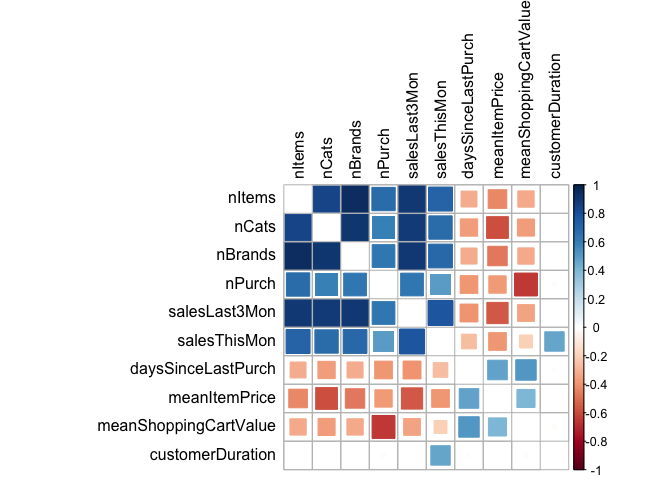
\includegraphics{Modeling-CLV_R-Markdown_files/figure-latex/unnamed-chunk-4-1.pdf}

Correlation for number of items orderd, number of brands, ncats, and
sales in last 3 months has positive strong correlation with sales.\\
We also observe somewhat positive correlation with customer druration to
sales

\hypertarget{make-a-box-plot-to-see-the-distribution-of-most-frequent-stores-and-preferred-brand}{%
\subsection{Make a box plot to see the distribution of most frequent
stores and preferred
brand}\label{make-a-box-plot-to-see-the-distribution-of-most-frequent-stores-and-preferred-brand}}

\hypertarget{most-frequent-stores}{%
\paragraph{Most frequent stores}\label{most-frequent-stores}}

\begin{Shaded}
\begin{Highlighting}[]
\KeywordTok{ggplot}\NormalTok{(}\DataTypeTok{data =}\NormalTok{ salesData, }\KeywordTok{aes}\NormalTok{(}\DataTypeTok{x =}\NormalTok{ mostFreqStore, }\DataTypeTok{y =}\NormalTok{ salesThisMon, }\DataTypeTok{color =}\NormalTok{ salesThisMon)) }\OperatorTok{+}
\StringTok{  }\KeywordTok{geom_boxplot}\NormalTok{(}\DataTypeTok{alpha =} \FloatTok{0.25}\NormalTok{) }\OperatorTok{+}
\StringTok{  }\KeywordTok{geom_jitter}\NormalTok{(}\DataTypeTok{shape =} \DecValTok{16}\NormalTok{, }\DataTypeTok{position =} \KeywordTok{position_jitter}\NormalTok{(}\FloatTok{0.2}\NormalTok{), }\DataTypeTok{size =} \FloatTok{1.5}\NormalTok{, }\DataTypeTok{alpha =} \FloatTok{0.7}\NormalTok{) }\OperatorTok{+}
\StringTok{  }\KeywordTok{scale_color_gradientn}\NormalTok{(}\DataTypeTok{name =} \StringTok{""}\NormalTok{, }\DataTypeTok{colours =} \KeywordTok{rev}\NormalTok{(viridis}\OperatorTok{::}\KeywordTok{viridis}\NormalTok{(}\DecValTok{20}\NormalTok{))) }\OperatorTok{+}
\StringTok{  }\KeywordTok{guides}\NormalTok{(}\DataTypeTok{color =}\NormalTok{ F)}
\end{Highlighting}
\end{Shaded}

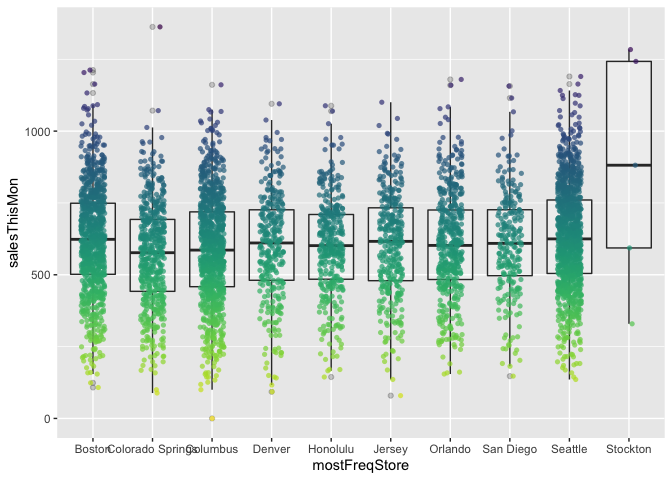
\includegraphics{Modeling-CLV_R-Markdown_files/figure-latex/unnamed-chunk-5-1.pdf}

\hypertarget{most-preferred-brands}{%
\paragraph{Most preferred brands}\label{most-preferred-brands}}

\begin{Shaded}
\begin{Highlighting}[]
\KeywordTok{ggplot}\NormalTok{(}\DataTypeTok{data =}\NormalTok{ salesData, }\KeywordTok{aes}\NormalTok{(}\DataTypeTok{x =}\NormalTok{ preferredBrand, }\DataTypeTok{y =}\NormalTok{ salesThisMon, }\DataTypeTok{color =}\NormalTok{ salesThisMon)) }\OperatorTok{+}
\StringTok{  }\KeywordTok{geom_boxplot}\NormalTok{(}\DataTypeTok{alpha =} \FloatTok{0.25}\NormalTok{) }\OperatorTok{+}
\StringTok{  }\KeywordTok{geom_jitter}\NormalTok{(}\DataTypeTok{shape =} \DecValTok{16}\NormalTok{, }\DataTypeTok{position =} \KeywordTok{position_jitter}\NormalTok{(}\FloatTok{0.2}\NormalTok{), }\DataTypeTok{size =} \FloatTok{1.5}\NormalTok{, }\DataTypeTok{alpha =} \FloatTok{0.7}\NormalTok{) }\OperatorTok{+}
\StringTok{  }\KeywordTok{scale_color_gradientn}\NormalTok{(}\DataTypeTok{name =} \StringTok{""}\NormalTok{, }\DataTypeTok{colours =} \KeywordTok{rev}\NormalTok{(viridis}\OperatorTok{::}\KeywordTok{viridis}\NormalTok{(}\DecValTok{20}\NormalTok{))) }\OperatorTok{+}
\StringTok{  }\KeywordTok{guides}\NormalTok{(}\DataTypeTok{color =}\NormalTok{ F) }
\end{Highlighting}
\end{Shaded}

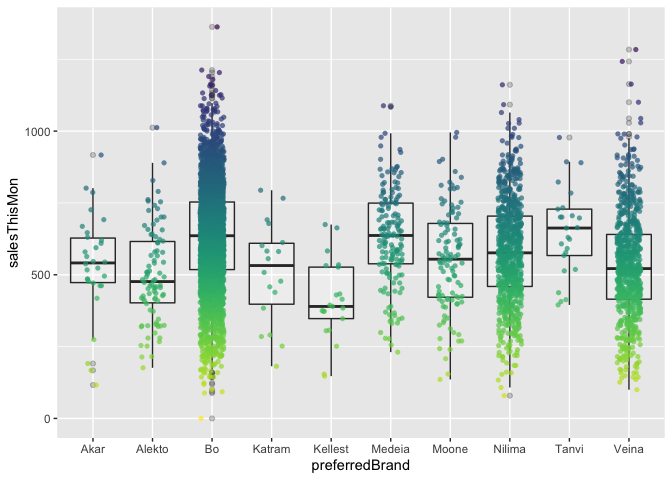
\includegraphics{Modeling-CLV_R-Markdown_files/figure-latex/unnamed-chunk-6-1.pdf}

\hypertarget{linear-regression-model}{%
\subsection{Linear Regression Model}\label{linear-regression-model}}

Now that we have looked at the correlation between variables, Let's
build a linear regression model

Lets start by building a simple linear regression model using sales in
the last 3 months as independent varioable since it has a strong
positive correlation with sales as observed in above correlation plot

\begin{Shaded}
\begin{Highlighting}[]
\NormalTok{salesSimpleModel =}\StringTok{ }\KeywordTok{lm}\NormalTok{(salesThisMon }\OperatorTok{~}\StringTok{ }\NormalTok{salesLast3Mon, }
                       \DataTypeTok{data =}\NormalTok{ salesData)}

\CommentTok{# Looking at model summary}
\KeywordTok{summary}\NormalTok{(salesSimpleModel)}
\end{Highlighting}
\end{Shaded}

\begin{verbatim}
## 
## Call:
## lm(formula = salesThisMon ~ salesLast3Mon, data = salesData)
## 
## Residuals:
##     Min      1Q  Median      3Q     Max 
## -570.18  -68.26    3.21   72.98  605.58 
## 
## Coefficients:
##                Estimate Std. Error t value Pr(>|t|)    
## (Intercept)   99.690501   6.083886   16.39   <2e-16 ***
## salesLast3Mon  0.382696   0.004429   86.40   <2e-16 ***
## ---
## Signif. codes:  0 '***' 0.001 '**' 0.01 '*' 0.05 '.' 0.1 ' ' 1
## 
## Residual standard error: 117.5 on 5120 degrees of freedom
## Multiple R-squared:  0.5932, Adjusted R-squared:  0.5931 
## F-statistic:  7465 on 1 and 5120 DF,  p-value: < 2.2e-16
\end{verbatim}

\begin{enumerate}
\def\labelenumi{\arabic{enumi}.}
\tightlist
\item
  The regression coeffecient of 0.38 means for every increase in sales
  of past 3 months, sales for this month will increase by 0.38 units.
\item
  And 59.3\% of change in sales for this month can be attributed to
  sales in past 3 months.
\end{enumerate}

\hypertarget{build-multiple-linear-regression-model}{%
\subsection{Build Multiple linear regression
model}\label{build-multiple-linear-regression-model}}

\begin{Shaded}
\begin{Highlighting}[]
\NormalTok{salesModel1 <-}\StringTok{ }\KeywordTok{lm}\NormalTok{(salesThisMon }\OperatorTok{~}\StringTok{ }\NormalTok{. }\OperatorTok{-}\StringTok{ }\NormalTok{id, }
                 \DataTypeTok{data =}\NormalTok{ salesData)}
\KeywordTok{summary}\NormalTok{(salesModel1)}
\end{Highlighting}
\end{Shaded}

\begin{verbatim}
## 
## Call:
## lm(formula = salesThisMon ~ . - id, data = salesData)
## 
## Residuals:
##     Min      1Q  Median      3Q     Max 
## -322.76  -50.76    0.78   50.90  398.79 
## 
## Coefficients:
##                                 Estimate Std. Error t value Pr(>|t|)    
## (Intercept)                   -2.585e+02  1.762e+01 -14.673  < 2e-16 ***
## nItems                         1.605e-01  2.709e-02   5.923 3.37e-09 ***
## mostFreqStoreColorado Springs -7.167e+00  4.350e+00  -1.648 0.099503 .  
## mostFreqStoreColumbus          9.579e-01  3.680e+00   0.260 0.794642    
## mostFreqStoreDenver           -8.601e+00  5.130e+00  -1.676 0.093722 .  
## mostFreqStoreHonolulu         -1.588e+01  4.916e+00  -3.231 0.001242 ** 
## mostFreqStoreJersey           -2.169e+01  5.031e+00  -4.311 1.66e-05 ***
## mostFreqStoreOrlando          -1.052e+01  4.492e+00  -2.342 0.019210 *  
## mostFreqStoreSan Diego        -2.009e+01  5.717e+00  -3.514 0.000446 ***
## mostFreqStoreSeattle          -9.784e+00  3.539e+00  -2.765 0.005716 ** 
## mostFreqStoreStockton         -1.176e+02  3.580e+01  -3.286 0.001022 ** 
## mostFreqCatBaby               -3.413e+00  3.513e+00  -0.972 0.331249    
## mostFreqCatBakery             -1.025e+01  5.456e+00  -1.879 0.060339 .  
## mostFreqCatBeverages           3.351e-01  7.008e+00   0.048 0.961867    
## mostFreqCatClothes            -8.527e+00  6.213e+00  -1.372 0.170010    
## mostFreqCatFresh food         -6.372e+00  7.245e+00  -0.880 0.379164    
## mostFreqCatFrozen food        -8.084e+00  3.840e+00  -2.105 0.035332 *  
## mostFreqCatPackaged food      -8.346e-01  4.356e+00  -0.192 0.848063    
## mostFreqCatPets                8.508e+00  7.242e+00   1.175 0.240102    
## mostFreqCatShoes               3.298e+00  3.286e+00   1.004 0.315452    
## nCats                         -7.917e-01  2.345e-01  -3.375 0.000742 ***
## preferredBrandAlekto          -5.590e+00  1.649e+01  -0.339 0.734645    
## preferredBrandBo              -2.505e+01  1.438e+01  -1.742 0.081516 .  
## preferredBrandKatram          -6.264e+01  2.334e+01  -2.684 0.007295 ** 
## preferredBrandKellest         -5.349e+01  2.214e+01  -2.416 0.015713 *  
## preferredBrandMedeia          -2.161e+01  1.556e+01  -1.389 0.164967    
## preferredBrandMoone           -4.166e+01  1.627e+01  -2.561 0.010453 *  
## preferredBrandNilima          -2.888e+01  1.454e+01  -1.986 0.047040 *  
## preferredBrandTanvi            3.135e+01  2.129e+01   1.472 0.141076    
## preferredBrandVeina           -1.861e+01  1.451e+01  -1.282 0.199837    
## nBrands                       -4.804e-02  8.468e-02  -0.567 0.570533    
## nPurch                         4.758e-01  1.513e-01   3.145 0.001669 ** 
## salesLast3Mon                  3.753e-01  8.599e-03  43.652  < 2e-16 ***
## daysSinceLastPurch             1.794e-01  1.524e-01   1.177 0.239322    
## meanItemPrice                  1.793e-01  9.289e-02   1.930 0.053680 .  
## meanShoppingCartValue          2.596e-01  2.618e-02   9.918  < 2e-16 ***
## customerDuration               5.713e-01  7.148e-03  79.927  < 2e-16 ***
## ---
## Signif. codes:  0 '***' 0.001 '**' 0.01 '*' 0.05 '.' 0.1 ' ' 1
## 
## Residual standard error: 77.34 on 5085 degrees of freedom
## Multiple R-squared:  0.8249, Adjusted R-squared:  0.8237 
## F-statistic: 665.6 on 36 and 5085 DF,  p-value: < 2.2e-16
\end{verbatim}

But one of the problem with multiple regression model is VIF. + check
VIF from ``car'' package and get rid of with one pair of variable with
VIF valuef of abve 10

\textbf{A variance inflation factor greater than 5 hints to
multicollinearity, greater than 10 indicates unstable regression
estimates.}

\begin{Shaded}
\begin{Highlighting}[]
\CommentTok{# library(car)}
\NormalTok{car}\OperatorTok{::}\KeywordTok{vif}\NormalTok{(salesModel1)}
\end{Highlighting}
\end{Shaded}

\begin{verbatim}
##                            GVIF Df GVIF^(1/(2*Df))
## nItems                11.772600  1        3.431122
## mostFreqStore          1.260469  9        1.012943
## mostFreqCat            1.527348  9        1.023809
## nCats                  8.402073  1        2.898633
## preferredBrand         1.682184  9        1.029316
## nBrands               14.150868  1        3.761764
## nPurch                 3.083952  1        1.756119
## salesLast3Mon          8.697663  1        2.949180
## daysSinceLastPurch     1.585057  1        1.258991
## meanItemPrice          1.987665  1        1.409846
## meanShoppingCartValue  2.247579  1        1.499193
## customerDuration       1.004664  1        1.002329
\end{verbatim}

Build another model by removing variables nItems and preferredBrand

\begin{Shaded}
\begin{Highlighting}[]
\NormalTok{salesModel2 <-}\StringTok{ }\KeywordTok{lm}\NormalTok{(salesThisMon }\OperatorTok{~}\StringTok{ }\NormalTok{. }\OperatorTok{-}\StringTok{ }\NormalTok{id }\OperatorTok{-}\StringTok{ }\NormalTok{nBrands }\OperatorTok{-}\StringTok{ }\NormalTok{preferredBrand, }
                 \DataTypeTok{data =}\NormalTok{ salesData)}
\KeywordTok{summary}\NormalTok{(salesModel2)}
\end{Highlighting}
\end{Shaded}

\begin{verbatim}
## 
## Call:
## lm(formula = salesThisMon ~ . - id - nBrands - preferredBrand, 
##     data = salesData)
## 
## Residuals:
##     Min      1Q  Median      3Q     Max 
## -322.66  -51.26    0.60   51.28  399.10 
## 
## Coefficients:
##                                 Estimate Std. Error t value Pr(>|t|)    
## (Intercept)                   -2.828e+02  1.007e+01 -28.079  < 2e-16 ***
## nItems                         1.470e-01  2.093e-02   7.023 2.45e-12 ***
## mostFreqStoreColorado Springs -7.829e+00  4.351e+00  -1.799 0.072047 .  
## mostFreqStoreColumbus          5.960e-01  3.682e+00   0.162 0.871391    
## mostFreqStoreDenver           -9.721e+00  5.133e+00  -1.894 0.058305 .  
## mostFreqStoreHonolulu         -1.604e+01  4.925e+00  -3.257 0.001134 ** 
## mostFreqStoreJersey           -2.215e+01  5.011e+00  -4.420 1.01e-05 ***
## mostFreqStoreOrlando          -1.104e+01  4.500e+00  -2.454 0.014154 *  
## mostFreqStoreSan Diego        -1.985e+01  5.718e+00  -3.472 0.000521 ***
## mostFreqStoreSeattle          -9.573e+00  3.542e+00  -2.702 0.006906 ** 
## mostFreqStoreStockton         -1.129e+02  3.559e+01  -3.171 0.001530 ** 
## mostFreqCatBaby               -3.496e+00  3.469e+00  -1.008 0.313594    
## mostFreqCatBakery             -9.908e+00  5.451e+00  -1.818 0.069188 .  
## mostFreqCatBeverages           9.253e-02  7.024e+00   0.013 0.989489    
## mostFreqCatClothes            -3.828e+00  6.090e+00  -0.629 0.529674    
## mostFreqCatFresh food         -5.935e+00  7.255e+00  -0.818 0.413368    
## mostFreqCatFrozen food        -7.196e+00  3.813e+00  -1.887 0.059179 .  
## mostFreqCatPackaged food      -1.387e+00  4.311e+00  -0.322 0.747746    
## mostFreqCatPets                9.073e+00  7.245e+00   1.252 0.210467    
## mostFreqCatShoes               2.649e+00  3.256e+00   0.814 0.415917    
## nCats                         -9.585e-01  1.956e-01  -4.900 9.90e-07 ***
## nPurch                         5.092e-01  1.513e-01   3.364 0.000773 ***
## salesLast3Mon                  3.782e-01  8.480e-03  44.604  < 2e-16 ***
## daysSinceLastPurch             1.712e-01  1.526e-01   1.122 0.262022    
## meanItemPrice                  2.253e-01  9.168e-02   2.457 0.014034 *  
## meanShoppingCartValue          2.584e-01  2.620e-02   9.861  < 2e-16 ***
## customerDuration               5.708e-01  7.162e-03  79.707  < 2e-16 ***
## ---
## Signif. codes:  0 '***' 0.001 '**' 0.01 '*' 0.05 '.' 0.1 ' ' 1
## 
## Residual standard error: 77.56 on 5095 degrees of freedom
## Multiple R-squared:  0.8236, Adjusted R-squared:  0.8227 
## F-statistic: 914.9 on 26 and 5095 DF,  p-value: < 2.2e-16
\end{verbatim}

\begin{Shaded}
\begin{Highlighting}[]
\KeywordTok{vif}\NormalTok{(salesModel2)}
\end{Highlighting}
\end{Shaded}

\begin{verbatim}
##                           GVIF Df GVIF^(1/(2*Df))
## nItems                6.987456  1        2.643380
## mostFreqStore         1.178251  9        1.009154
## mostFreqCat           1.269636  9        1.013351
## nCats                 5.813494  1        2.411119
## nPurch                3.069046  1        1.751869
## salesLast3Mon         8.412520  1        2.900435
## daysSinceLastPurch    1.579426  1        1.256752
## meanItemPrice         1.925494  1        1.387622
## meanShoppingCartValue 2.238410  1        1.496132
## customerDuration      1.002981  1        1.001489
\end{verbatim}

\hypertarget{now-its-time-for-model-validation-model-fit-and-prediction}{%
\subsection{Now, it's time for model validation, model fit, and
prediction}\label{now-its-time-for-model-validation-model-fit-and-prediction}}

\emph{F test is the test used to validate the model} In our salesModel2,
the value of p is less tha 0.05 and hence, the hypothesis of Rsquare
equal to 0 is rejected

\hypertarget{method-to-avoid-overfitting}{%
\paragraph{Method to avoid
overfitting:}\label{method-to-avoid-overfitting}}

\begin{enumerate}
\def\labelenumi{\arabic{enumi}.}
\tightlist
\item
  AIC() from stats package - useful whe comparing two or more models
\item
  stepAIC() from MASS package
\item
  out-of-sample model validation
\item
  cross-validation
\end{enumerate}

\hypertarget{predcict-the-sales-and-calculate-ite-mean-on-new-data-set}{%
\subsubsection{Predcict the sales and calculate it'e mean on new data
set}\label{predcict-the-sales-and-calculate-ite-mean-on-new-data-set}}

\begin{Shaded}
\begin{Highlighting}[]
\CommentTok{# load new data set}
\NormalTok{salesData2_}\DecValTok{4}\NormalTok{ =}\StringTok{ }\KeywordTok{read.csv}\NormalTok{(}\StringTok{"/Users/bhavinghoghari/Desktop/Work/Self Learn/R/Marketing Analytics in R/Data Camp_Data sets/salesDataMon2To4.csv"}\NormalTok{)}

\CommentTok{# use predict () function on new data set}
\NormalTok{predictSales5 =}\StringTok{ }\KeywordTok{predict}\NormalTok{(salesModel2, }\DataTypeTok{newdata =}\NormalTok{ salesData2_}\DecValTok{4}\NormalTok{)}

\CommentTok{# calculate mean}
\KeywordTok{mean}\NormalTok{(predictSales5)}
\end{Highlighting}
\end{Shaded}

\begin{verbatim}
## [1] 625.1438
\end{verbatim}

\hypertarget{churn-prevention}{%
\section{Churn Prevention}\label{churn-prevention}}

\hypertarget{using-logistic-regression}{%
\subsubsection{Using Logistic
Regression}\label{using-logistic-regression}}

\begin{Shaded}
\begin{Highlighting}[]
\CommentTok{# Load required file}
\NormalTok{defaultData =}\StringTok{ }\KeywordTok{read.csv}\NormalTok{(}\StringTok{"/Users/bhavinghoghari/Desktop/Work/Self Learn/R/Marketing Analytics in R/Data Camp_Data sets/defaultData.csv"}\NormalTok{, }\DataTypeTok{header =}\NormalTok{ T, }\DataTypeTok{sep =} \StringTok{";"}\NormalTok{)}

\KeywordTok{glimpse}\NormalTok{(defaultData)}
\end{Highlighting}
\end{Shaded}

\begin{verbatim}
## Observations: 18,000
## Variables: 25
## $ ID             <int> 1, 2, 3, 4, 5, 6, 7, 8, 9, 10, 11, 12, 13, 14, 15, 1...
## $ limitBal       <int> 20000, 120000, 90000, 50000, 50000, 50000, 500000, 1...
## $ sex            <int> 2, 2, 2, 2, 1, 1, 1, 2, 2, 1, 2, 2, 2, 1, 1, 2, 1, 1...
## $ education      <int> 2, 2, 2, 2, 2, 1, 1, 2, 3, 3, 3, 1, 2, 2, 1, 3, 1, 1...
## $ marriage       <int> 1, 2, 2, 1, 1, 2, 2, 2, 1, 2, 2, 2, 2, 2, 2, 3, 2, 1...
## $ age            <int> 24, 26, 34, 37, 57, 37, 29, 23, 28, 35, 34, 51, 41, ...
## $ pay1           <int> 2, -1, 0, 0, -1, 0, 0, 0, 0, -2, 0, -1, -1, 1, 0, 1,...
## $ pay2           <int> 2, 2, 0, 0, 0, 0, 0, -1, 0, -2, 0, -1, 0, 2, 0, 2, 0...
## $ pay3           <int> -1, 0, 0, 0, -1, 0, 0, -1, 2, -2, 2, -1, -1, 2, 0, 0...
## $ pay4           <int> -1, 0, 0, 0, 0, 0, 0, 0, 0, -2, 0, -1, -1, 0, 0, 0, ...
## $ pay5           <int> -2, 0, 0, 0, 0, 0, 0, 0, 0, -1, 0, -1, -1, 0, 0, 0, ...
## $ pay6           <int> -2, 2, 0, 0, 0, 0, 0, -1, 0, -1, -1, 2, -1, 2, 0, 0,...
## $ billAmt1       <int> 3913, 2682, 29239, 46990, 8617, 64400, 367965, 11876...
## $ billAmt2       <int> 3102, 1725, 14027, 48233, 5670, 57069, 412023, 380, ...
## $ billAmt3       <int> 689, 2682, 13559, 49291, 35835, 57608, 445007, 601, ...
## $ billAmt4       <int> 0, 3272, 14331, 28314, 20940, 19394, 542653, 221, 12...
## $ billAmt5       <int> 0, 3455, 14948, 28959, 19146, 19619, 483003, -159, 1...
## $ billAmt6       <int> 0, 3261, 15549, 29547, 19131, 20024, 473944, 567, 37...
## $ payAmt1        <int> 0, 0, 1518, 2000, 2000, 2500, 55000, 380, 3329, 0, 2...
## $ payAmt2        <int> 689, 1000, 1500, 2019, 36681, 1815, 40000, 601, 0, 0...
## $ payAmt3        <int> 0, 1000, 1000, 1200, 10000, 657, 38000, 0, 432, 0, 5...
## $ payAmt4        <int> 0, 1000, 1000, 1100, 9000, 1000, 20239, 581, 1000, 1...
## $ payAmt5        <int> 0, 0, 1000, 1069, 689, 1000, 13750, 1687, 1000, 1122...
## $ payAmt6        <int> 0, 2000, 5000, 1000, 679, 800, 13770, 1542, 1000, 0,...
## $ PaymentDefault <int> 1, 1, 0, 0, 0, 0, 0, 0, 0, 0, 0, 0, 0, 1, 0, 0, 1, 0...
\end{verbatim}

Get some more insights about the variable of interest PaymentDefault by
plotting a bar chart of the two levels.

\begin{Shaded}
\begin{Highlighting}[]
\KeywordTok{ggplot}\NormalTok{(}\DataTypeTok{data =}\NormalTok{ defaultData, }\KeywordTok{aes}\NormalTok{(}\DataTypeTok{x =}\NormalTok{ PaymentDefault,)) }\OperatorTok{+}
\StringTok{  }\KeywordTok{geom_histogram}\NormalTok{(}\DataTypeTok{stat =} \StringTok{"count"}\NormalTok{)}
\end{Highlighting}
\end{Shaded}

\begin{verbatim}
## Warning: Ignoring unknown parameters: binwidth, bins, pad
\end{verbatim}

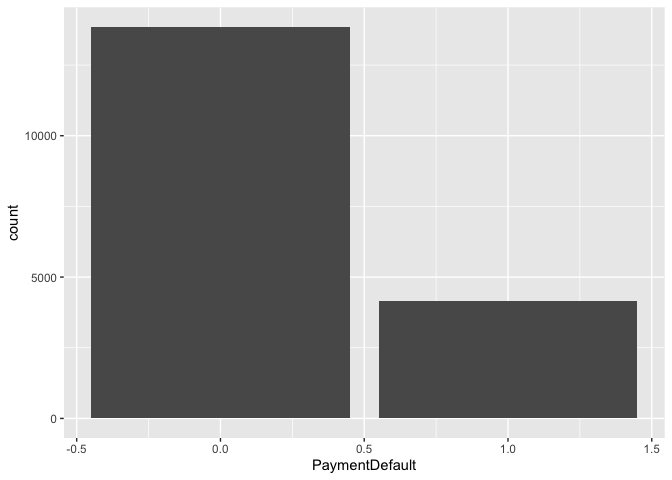
\includegraphics{Modeling-CLV_R-Markdown_files/figure-latex/unnamed-chunk-13-1.pdf}

\hypertarget{logistic-regression-model}{%
\paragraph{Logistic Regression Model}\label{logistic-regression-model}}

\hypertarget{how-does-hypothesis-test-actually-works}{%
\subparagraph{How does hypothesis test actually
works?}\label{how-does-hypothesis-test-actually-works}}

When we draw a curve on graph for 0 and 1, we see the value is towards
the end of tail of 0, then the null hypothesis is more like to be proven
void.

\hypertarget{model-selection}{%
\paragraph{Model Selection}\label{model-selection}}

It is important to understand which variables to include in the model.
One of the few method is to use ``stepAIC()'' from package ``mass''. +
This method uses selects and drops all variable simantaniously until the
AIC value of model drops to lowest possible value

\begin{Shaded}
\begin{Highlighting}[]
\CommentTok{# build a logistic regression model}
\NormalTok{logitModelFull <-}\StringTok{ }\KeywordTok{glm}\NormalTok{(PaymentDefault }\OperatorTok{~}\StringTok{ }\NormalTok{limitBal }\OperatorTok{+}\StringTok{ }\NormalTok{sex }\OperatorTok{+}\StringTok{ }\NormalTok{education }\OperatorTok{+}\StringTok{ }\NormalTok{marriage }\OperatorTok{+}
\StringTok{                   }\NormalTok{age }\OperatorTok{+}\StringTok{ }\NormalTok{pay1 }\OperatorTok{+}\StringTok{ }\NormalTok{pay2 }\OperatorTok{+}\StringTok{ }\NormalTok{pay3 }\OperatorTok{+}\StringTok{ }\NormalTok{pay4 }\OperatorTok{+}\StringTok{ }\NormalTok{pay5 }\OperatorTok{+}\StringTok{ }\NormalTok{pay6 }\OperatorTok{+}\StringTok{ }\NormalTok{billAmt1 }\OperatorTok{+}\StringTok{ }
\StringTok{                   }\NormalTok{billAmt2 }\OperatorTok{+}\StringTok{ }\NormalTok{billAmt3 }\OperatorTok{+}\StringTok{ }\NormalTok{billAmt4 }\OperatorTok{+}\StringTok{ }\NormalTok{billAmt5 }\OperatorTok{+}\StringTok{ }\NormalTok{billAmt6 }\OperatorTok{+}\StringTok{ }\NormalTok{payAmt1 }\OperatorTok{+}\StringTok{ }
\StringTok{                   }\NormalTok{payAmt2 }\OperatorTok{+}\StringTok{ }\NormalTok{payAmt3 }\OperatorTok{+}\StringTok{ }\NormalTok{payAmt4 }\OperatorTok{+}\StringTok{ }\NormalTok{payAmt5 }\OperatorTok{+}\StringTok{ }\NormalTok{payAmt6, }
                 \DataTypeTok{family =}\NormalTok{ binomial, }\DataTypeTok{data =}\NormalTok{ defaultData)}

\CommentTok{# Take a look at the model}
\KeywordTok{summary}\NormalTok{(logitModelFull)}
\end{Highlighting}
\end{Shaded}

\begin{verbatim}
## 
## Call:
## glm(formula = PaymentDefault ~ limitBal + sex + education + marriage + 
##     age + pay1 + pay2 + pay3 + pay4 + pay5 + pay6 + billAmt1 + 
##     billAmt2 + billAmt3 + billAmt4 + billAmt5 + billAmt6 + payAmt1 + 
##     payAmt2 + payAmt3 + payAmt4 + payAmt5 + payAmt6, family = binomial, 
##     data = defaultData)
## 
## Deviance Residuals: 
##     Min       1Q   Median       3Q      Max  
## -3.0893  -0.7116  -0.5615  -0.2794   4.2501  
## 
## Coefficients:
##               Estimate Std. Error z value Pr(>|z|)    
## (Intercept) -5.711e-01  1.505e-01  -3.795 0.000148 ***
## limitBal    -4.825e-07  1.985e-07  -2.431 0.015052 *  
## sex         -8.251e-02  3.880e-02  -2.127 0.033457 *  
## education   -1.217e-01  2.745e-02  -4.434 9.23e-06 ***
## marriage    -1.711e-01  4.016e-02  -4.259 2.05e-05 ***
## age          4.824e-03  2.257e-03   2.137 0.032570 *  
## pay1         5.743e-01  2.221e-02  25.864  < 2e-16 ***
## pay2         5.156e-02  2.552e-02   2.020 0.043336 *  
## pay3         7.811e-02  2.863e-02   2.728 0.006375 ** 
## pay4        -1.191e-02  3.285e-02  -0.363 0.716838    
## pay5         1.080e-01  3.381e-02   3.193 0.001406 ** 
## pay6        -1.956e-02  2.750e-02  -0.711 0.476852    
## billAmt1    -7.948e-06  1.582e-06  -5.023 5.09e-07 ***
## billAmt2     4.911e-06  2.006e-06   2.448 0.014350 *  
## billAmt3     4.203e-07  1.698e-06   0.247 0.804572    
## billAmt4    -1.587e-08  1.872e-06  -0.008 0.993234    
## billAmt5     9.703e-07  2.154e-06   0.451 0.652293    
## billAmt6     6.758e-07  1.591e-06   0.425 0.670955    
## payAmt1     -1.878e-05  3.252e-06  -5.777 7.61e-09 ***
## payAmt2     -6.406e-06  2.364e-06  -2.710 0.006731 ** 
## payAmt3     -3.325e-06  2.401e-06  -1.385 0.166153    
## payAmt4     -3.922e-06  2.342e-06  -1.675 0.093970 .  
## payAmt5     -2.383e-06  2.168e-06  -1.099 0.271635    
## payAmt6     -1.916e-06  1.618e-06  -1.184 0.236521    
## ---
## Signif. codes:  0 '***' 0.001 '**' 0.01 '*' 0.05 '.' 0.1 ' ' 1
## 
## (Dispersion parameter for binomial family taken to be 1)
## 
##     Null deviance: 19438  on 17999  degrees of freedom
## Residual deviance: 17216  on 17976  degrees of freedom
## AIC: 17264
## 
## Number of Fisher Scoring iterations: 5
\end{verbatim}

Extract the coefficients from the model, then transform them to the odds
ratios and round \emph{By applying the exp() function to the
coefficients (coef()) of the logit model, you can get to the effects on
the odds (odds ratios).}

\begin{Shaded}
\begin{Highlighting}[]
\CommentTok{# Take a look at the odds ratios}
\NormalTok{coefsexp <-}\StringTok{ }\KeywordTok{coef}\NormalTok{(logitModelFull) }\OperatorTok\StringTok{ }\KeywordTok{exp}\NormalTok{() }\OperatorTok\StringTok{ }\KeywordTok{round}\NormalTok{(}\DecValTok{2}\NormalTok{)}
\NormalTok{coefsexp}
\end{Highlighting}
\end{Shaded}

\begin{verbatim}
## (Intercept)    limitBal         sex   education    marriage         age 
##        0.56        1.00        0.92        0.89        0.84        1.00 
##        pay1        pay2        pay3        pay4        pay5        pay6 
##        1.78        1.05        1.08        0.99        1.11        0.98 
##    billAmt1    billAmt2    billAmt3    billAmt4    billAmt5    billAmt6 
##        1.00        1.00        1.00        1.00        1.00        1.00 
##     payAmt1     payAmt2     payAmt3     payAmt4     payAmt5     payAmt6 
##        1.00        1.00        1.00        1.00        1.00        1.00
\end{verbatim}

Checking the odds ratio helps us get a direction of effect of
independent variables to dependent variables \textgreater{} The above
result shows that married people are more likely to buy back by factor
of 0.84 compared to somebody who is not marrried.

\hypertarget{build-another-model-using-stepaic-and-see-the-difference-in-aic-value}{%
\paragraph{Build another model using stepAIC() and see the difference in
AIC
value}\label{build-another-model-using-stepaic-and-see-the-difference-in-aic-value}}

load required package ``MASS''

\begin{Shaded}
\begin{Highlighting}[]
\CommentTok{# library(MASS)}
\CommentTok{# Set trace = 0, as you do not want to get an output for the whole model selection process. Save the result to the object logitModelNew}
\NormalTok{logitModelNew <-}\StringTok{ }\KeywordTok{stepAIC}\NormalTok{(logitModelFull, }\DataTypeTok{trace =} \DecValTok{0}\NormalTok{)}

\KeywordTok{summary}\NormalTok{(logitModelNew)}
\end{Highlighting}
\end{Shaded}

\begin{verbatim}
## 
## Call:
## glm(formula = PaymentDefault ~ limitBal + sex + education + marriage + 
##     age + pay1 + pay2 + pay3 + pay5 + billAmt1 + billAmt2 + billAmt5 + 
##     payAmt1 + payAmt2 + payAmt3 + payAmt4, family = binomial, 
##     data = defaultData)
## 
## Deviance Residuals: 
##     Min       1Q   Median       3Q      Max  
## -3.0839  -0.7119  -0.5611  -0.2839   4.1800  
## 
## Coefficients:
##               Estimate Std. Error z value Pr(>|z|)    
## (Intercept) -5.699e-01  1.504e-01  -3.790 0.000151 ***
## limitBal    -5.201e-07  1.954e-07  -2.661 0.007791 ** 
## sex         -8.206e-02  3.878e-02  -2.116 0.034338 *  
## education   -1.212e-01  2.744e-02  -4.418 9.96e-06 ***
## marriage    -1.724e-01  4.014e-02  -4.295 1.75e-05 ***
## age          4.863e-03  2.256e-03   2.156 0.031092 *  
## pay1         5.740e-01  2.218e-02  25.882  < 2e-16 ***
## pay2         4.979e-02  2.552e-02   1.951 0.051048 .  
## pay3         7.197e-02  2.573e-02   2.798 0.005146 ** 
## pay5         8.859e-02  2.249e-02   3.938 8.20e-05 ***
## billAmt1    -8.130e-06  1.580e-06  -5.144 2.69e-07 ***
## billAmt2     5.238e-06  1.775e-06   2.951 0.003165 ** 
## billAmt5     1.790e-06  8.782e-07   2.038 0.041554 *  
## payAmt1     -1.931e-05  3.258e-06  -5.928 3.06e-09 ***
## payAmt2     -6.572e-06  2.092e-06  -3.142 0.001681 ** 
## payAmt3     -3.693e-06  2.187e-06  -1.689 0.091241 .  
## payAmt4     -4.611e-06  2.062e-06  -2.237 0.025306 *  
## ---
## Signif. codes:  0 '***' 0.001 '**' 0.01 '*' 0.05 '.' 0.1 ' ' 1
## 
## (Dispersion parameter for binomial family taken to be 1)
## 
##     Null deviance: 19438  on 17999  degrees of freedom
## Residual deviance: 17220  on 17983  degrees of freedom
## AIC: 17254
## 
## Number of Fisher Scoring iterations: 5
\end{verbatim}

The formula is saved in an object so that you don't have to type the
whole equation again when you want to use it later.

\begin{Shaded}
\begin{Highlighting}[]
\CommentTok{# Save the formula of the new model (it will be needed for the out-of-sample part) }
\NormalTok{formulaLogit <-}\StringTok{ }\KeywordTok{as.formula}\NormalTok{(}\KeywordTok{summary}\NormalTok{(logitModelNew)}\OperatorTok{$}\NormalTok{call)}
\NormalTok{formulaLogit}
\end{Highlighting}
\end{Shaded}

\begin{verbatim}
## PaymentDefault ~ limitBal + sex + education + marriage + age + 
##     pay1 + pay2 + pay3 + pay5 + billAmt1 + billAmt2 + billAmt5 + 
##     payAmt1 + payAmt2 + payAmt3 + payAmt4
\end{verbatim}

\hypertarget{in-sample-model-fit-and-thresholding}{%
\paragraph{In-Sample model fit and
Thresholding}\label{in-sample-model-fit-and-thresholding}}

\hypertarget{ways-to-measure-the-accuracy-and-validation-of-model}{%
\paragraph{Ways to measure the accuracy and validation of
model}\label{ways-to-measure-the-accuracy-and-validation-of-model}}

\hypertarget{similar-to-r-square-in-linear-regression-in-logistic-regression-we-use-pseudo-r-square-statistics.}{%
\subparagraph{1. Similar to R square in linear regression, in logistic
regression we use Pseudo R square
statistics.}\label{similar-to-r-square-in-linear-regression-in-logistic-regression-we-use-pseudo-r-square-statistics.}}

This includes: 1. McFadden, 2. Cox \& Snell 3. Nagelkerke

Interpretation - For this method, 1. \textbf{Reasonable \textgreater{}
0.2} value of 0.2 or higher is resonable 2. \textbf{Good if
\textgreater{} 0.4} value of 0.4 or higher is considered good 3.
\textbf{Very Good if \textgreater{} 0.5} value of 0.5 or higher is
considered to be very good

Package ``descr'' and function LogRegR2() gives us a value of Pseudo R2
for above three methods. \emph{Garbage in, Garbage out} \emph{model can
only be as good as the data}

\hypertarget{another-way-to-test-the-accuracy-of-model-is-to-use-predict-to-predict-the-future-values-using-type-response-and-compare-it-against-the-actual-values}{%
\subparagraph{2. Another way to test the accuracy of model is to use
predict() to predict the future values using type = ``response'' and
compare it against the actual
values}\label{another-way-to-test-the-accuracy-of-model-is-to-use-predict-to-predict-the-future-values-using-type-response-and-compare-it-against-the-actual-values}}

\hypertarget{another-test-is-to-use-confusion-matrix-from-package-sdmtools}{%
\subparagraph{3. Another test is to use confusion matrix from package
"SDMTools:}\label{another-test-is-to-use-confusion-matrix-from-package-sdmtools}}

\emph{note that SDMTools cannot be downloaded from CRAN anymore. Install
it instead it via ''`\{r\}remote::install\_version(``SDMTools'',
``1.1-221'')'''}

\hypertarget{checking-the-accuracy-of-of-model}{%
\subparagraph{Checking the accuracy of of
model}\label{checking-the-accuracy-of-of-model}}

It is not always correct to check the accuracy or mean of predicted to
actual values since the model might accurately predict that more
customers would not return but it does also predict that more customers
would return while in actual only few customers actually returned.

Hence, finding the right threshold is necessary to acheive the highest
possible payoff even though it means decrease in model accuracy rate.

\begin{Shaded}
\begin{Highlighting}[]
\CommentTok{# calculate prediction using predict() on logitModelFull}
\NormalTok{defaultData}\OperatorTok{$}\NormalTok{predFull =}\StringTok{ }\KeywordTok{predict}\NormalTok{(logitModelFull, }\DataTypeTok{type =} \StringTok{"response"}\NormalTok{, }\DataTypeTok{na.action =}\NormalTok{ na.exclude)}
\end{Highlighting}
\end{Shaded}

Now build a confusion matrix from package ``caret'' to see the accuracy
of the model \emph{make sure that the string type is set to factor for
actual values and predicted values}

\begin{Shaded}
\begin{Highlighting}[]
\CommentTok{# set a threshold of 0.5 and convert it to integer to match with the actual values class}
\NormalTok{defaultData}\OperatorTok{$}\NormalTok{predFull_}\FloatTok{0.5}\NormalTok{ =}\StringTok{ }\KeywordTok{as.integer}\NormalTok{(}\KeywordTok{ifelse}\NormalTok{(defaultData}\OperatorTok{$}\NormalTok{predFull }\OperatorTok{>=}\StringTok{ }\FloatTok{0.5}\NormalTok{, }\DecValTok{1}\NormalTok{, }\DecValTok{0}\NormalTok{))}

\CommentTok{# create a confusion matrix using package "caret" and set both string to factor class}
\CommentTok{# library(caret)}
\NormalTok{confMatrixModelFull =}\StringTok{ }\KeywordTok{confusionMatrix}\NormalTok{(}\KeywordTok{as.factor}\NormalTok{(defaultData}\OperatorTok{$}\NormalTok{PaymentDefault), }\KeywordTok{as.factor}\NormalTok{(defaultData}\OperatorTok{$}\NormalTok{predFull_}\FloatTok{0.5}\NormalTok{))}
\NormalTok{confMatrixModelFull}
\end{Highlighting}
\end{Shaded}

\begin{verbatim}
##      [,1]  [,2]
## [1,]    0     0
## [2,]    0 13850
\end{verbatim}

Since we calculated the accuracy for confMatrixModelFull, also let's
calculate accuracy for logitModelNew which we built above usinf stepAIC

First step is to: 1. Predict the probability using predict function and
set type = ``response'' 2. Set a desired threshold and mutate value to
new column 3. Create confusion matrix

\begin{Shaded}
\begin{Highlighting}[]
\CommentTok{# predict the values}
\NormalTok{defaultData}\OperatorTok{$}\NormalTok{predNew =}\StringTok{ }\KeywordTok{predict}\NormalTok{(logitModelNew, }\DataTypeTok{type =} \StringTok{"response"}\NormalTok{, }\DataTypeTok{na.action =}\NormalTok{ na.exclude)}

\CommentTok{# set threshold and convert values to 1,0}
\NormalTok{defaultData}\OperatorTok{$}\NormalTok{predNew_}\FloatTok{0.5}\NormalTok{ =}\StringTok{ }\KeywordTok{as.integer}\NormalTok{(}\KeywordTok{ifelse}\NormalTok{(defaultData}\OperatorTok{$}\NormalTok{predNew }\OperatorTok{>=}\StringTok{ }\FloatTok{0.5}\NormalTok{, }\DecValTok{1}\NormalTok{, }\DecValTok{0}\NormalTok{))}

\CommentTok{# create a confusion matrix using package "caret" and set both string to factor class}
\CommentTok{# library(caret)}
\NormalTok{confMatrixModelNew =}\StringTok{ }\KeywordTok{confusionMatrix}\NormalTok{(}\KeywordTok{as.factor}\NormalTok{(defaultData}\OperatorTok{$}\NormalTok{PaymentDefault), }\KeywordTok{as.factor}\NormalTok{(defaultData}\OperatorTok{$}\NormalTok{predNew_}\FloatTok{0.5}\NormalTok{))}
\NormalTok{confMatrixModelNew}
\end{Highlighting}
\end{Shaded}

\begin{verbatim}
##      [,1]  [,2]
## [1,]    0     0
## [2,]    0 13850
\end{verbatim}

From the above confusion matrix: 1. \textbf{True Positive} - We
correctly predicted that customer would default = 998 2. \textbf{True
Negative} - We correctly predicted that customer would not default =
13443 3. \textbf{False Positive} - We incorrectly predicted that
customer would default = 3152 4. \textbf{False Negative} - We
incorrectly predicted that customer would not default = 407

\hypertarget{finding-the-optimal-threshold-is-important}{%
\paragraph{Finding the optimal threshold is
important}\label{finding-the-optimal-threshold-is-important}}

Imagine you are running a campaign with the aim of preventing customers
to default. You can lay out your campaign with the help of your
predictions. Thereby, the choice of the threshold is essential for your
results. If you know the costs and the rewards of your campaign, you can
empirically check which threshold is most reasonable. In this exercise,
we are faced with the following scenario:

If a customer does not default due to our campaign, i.e.~if we predicted
the default correctly (true positive) we are rewarded with 1000€. If
however we aim our campaign at a customer who would not have defaulted
anyways, i.e.~if we falsely predicted the customer (false positive) to
default, we are faced with costs of 250€.

From the last exercise we know that the restricted model was the best
one. So only calculate the optimal threshold for that model.

\begin{Shaded}
\begin{Highlighting}[]
\CommentTok{# create a confusion matrix for actual vs predicted}
\NormalTok{confusionMatrix_tableNew_}\FloatTok{0.5}\NormalTok{ =}\StringTok{ }\KeywordTok{confusionMatrix}\NormalTok{(defaultData}\OperatorTok{$}\NormalTok{PaymentDefault, defaultData}\OperatorTok{$}\NormalTok{predNew_}\FloatTok{0.5}\NormalTok{)}

\CommentTok{# Now }
\NormalTok{payoff_}\FloatTok{0.5}\NormalTok{ =}\StringTok{ }\DecValTok{1000}\OperatorTok{*}\NormalTok{confusionMatrix_tableNew_}\FloatTok{0.5}\NormalTok{[}\DecValTok{2}\NormalTok{,}\DecValTok{2}\NormalTok{] }\OperatorTok{-}\StringTok{ }\DecValTok{250}\OperatorTok{*}\NormalTok{confusionMatrix_tableNew_}\FloatTok{0.5}\NormalTok{[}\DecValTok{2}\NormalTok{,}\DecValTok{1}\NormalTok{]}
\NormalTok{payoff_}\FloatTok{0.5}
\end{Highlighting}
\end{Shaded}

\begin{verbatim}
## [1] 896250
\end{verbatim}

\hypertarget{below-we-now-create}{%
\paragraph{Below we now create}\label{below-we-now-create}}

\begin{enumerate}
\def\labelenumi{\arabic{enumi}.}
\tightlist
\item
  Predicted column for each threshold from 0.1 - 0.5
\item
  Then create confusion matrix table for each preeicted threshold values
\item
  Calculate payoff from each table. The value of 1000 is reward for
  calculating the \textbf{True Positve} value and 250 is penalty for
  \textbf{False Positive} values. \emph{Value of 1000 and 250 is based
  on knowing the value of customer. It can be changed according to
  business}
\end{enumerate}

\begin{Shaded}
\begin{Highlighting}[]
\CommentTok{# create a payoffmatrix for different threshold using loop}
\NormalTok{payoffmatrix_usingLoopFunction =}\StringTok{ }\KeywordTok{data.frame}\NormalTok{(}\DataTypeTok{threshold =} \KeywordTok{c}\NormalTok{(}\FloatTok{0.1}\NormalTok{,}\FloatTok{0.2}\NormalTok{,}\FloatTok{0.3}\NormalTok{,}\FloatTok{0.4}\NormalTok{,}\FloatTok{0.5}\NormalTok{), }
                                            \DataTypeTok{payoff =} \KeywordTok{c}\NormalTok{(}\OtherTok{NA}\NormalTok{,}\OtherTok{NA}\NormalTok{,}\OtherTok{NA}\NormalTok{,}\OtherTok{NA}\NormalTok{,}\OtherTok{NA}\NormalTok{))}

\CommentTok{# Set up the loop}
\ControlFlowTok{for}\NormalTok{(i }\ControlFlowTok{in} \DecValTok{1}\OperatorTok{:}\DecValTok{5}\NormalTok{) \{}
  \CommentTok{# Calculate specific confusion matrix with respective threshold}
\NormalTok{  confMatrix <-}\StringTok{ }\KeywordTok{confusionMatrix}\NormalTok{(defaultData}\OperatorTok{$}\NormalTok{PaymentDefault,}
\NormalTok{                defaultData}\OperatorTok{$}\NormalTok{predNew, }
                \DataTypeTok{cutoff =}\NormalTok{ payoffmatrix_usingLoopFunction}\OperatorTok{$}\NormalTok{threshold[i])}
  \CommentTok{# Calculate payoff and save it to the corresponding row}
\NormalTok{  payoffmatrix_usingLoopFunction}\OperatorTok{$}\NormalTok{payoff[i] <-}\StringTok{ }\DecValTok{1000}\OperatorTok{*}\NormalTok{confMatrix[}\DecValTok{2}\NormalTok{,}\DecValTok{2}\NormalTok{] }\OperatorTok{-}\StringTok{ }\DecValTok{250}\OperatorTok{*}\NormalTok{confMatrix[}\DecValTok{2}\NormalTok{,}\DecValTok{1}\NormalTok{]}
\NormalTok{\}}
\NormalTok{payoffmatrix_usingLoopFunction}
\end{Highlighting}
\end{Shaded}

\begin{verbatim}
##   threshold  payoff
## 1       0.1  994250
## 2       0.2 1440250
## 3       0.3 1575500
## 4       0.4 1328750
## 5       0.5  896250
\end{verbatim}

\begin{quote}
Threshold of 0.3 seems to be payoff maximum hence, we will use 0.3 as
our cutoff/threshold
\end{quote}

\emph{Another way of calculating threshold is by creating a predictive
column for each threshold}

\begin{Shaded}
\begin{Highlighting}[]
\KeywordTok{str}\NormalTok{(defaultData}\OperatorTok{$}\NormalTok{predNew_}\FloatTok{0.2}\NormalTok{)}
\end{Highlighting}
\end{Shaded}

\begin{verbatim}
##  NULL
\end{verbatim}

\begin{Shaded}
\begin{Highlighting}[]
\NormalTok{defaultData}\OperatorTok{$}\NormalTok{predNew_}\FloatTok{0.1}\NormalTok{ =}\StringTok{ }\KeywordTok{as.integer}\NormalTok{(}\KeywordTok{ifelse}\NormalTok{(defaultData}\OperatorTok{$}\NormalTok{predNew }\OperatorTok{>}\StringTok{ }\FloatTok{0.1}\NormalTok{, }\DecValTok{1}\NormalTok{, }\DecValTok{0}\NormalTok{))}
\NormalTok{defaultData}\OperatorTok{$}\NormalTok{predNew_}\FloatTok{0.2}\NormalTok{ =}\StringTok{ }\KeywordTok{as.integer}\NormalTok{(}\KeywordTok{ifelse}\NormalTok{(defaultData}\OperatorTok{$}\NormalTok{predNew }\OperatorTok{>}\StringTok{ }\FloatTok{0.2}\NormalTok{, }\DecValTok{1}\NormalTok{, }\DecValTok{0}\NormalTok{))}
\NormalTok{defaultData}\OperatorTok{$}\NormalTok{predNew_}\FloatTok{0.3}\NormalTok{ =}\StringTok{ }\KeywordTok{as.integer}\NormalTok{(}\KeywordTok{ifelse}\NormalTok{(defaultData}\OperatorTok{$}\NormalTok{predNew }\OperatorTok{>}\StringTok{ }\FloatTok{0.3}\NormalTok{, }\DecValTok{1}\NormalTok{, }\DecValTok{0}\NormalTok{))}
\NormalTok{defaultData}\OperatorTok{$}\NormalTok{predNew_}\FloatTok{0.4}\NormalTok{ =}\StringTok{ }\KeywordTok{as.integer}\NormalTok{(}\KeywordTok{ifelse}\NormalTok{(defaultData}\OperatorTok{$}\NormalTok{predNew }\OperatorTok{>}\StringTok{ }\FloatTok{0.4}\NormalTok{, }\DecValTok{1}\NormalTok{, }\DecValTok{0}\NormalTok{))}
\NormalTok{defaultData}\OperatorTok{$}\NormalTok{predNew_}\FloatTok{0.5}\NormalTok{ =}\StringTok{ }\KeywordTok{as.integer}\NormalTok{(}\KeywordTok{ifelse}\NormalTok{(defaultData}\OperatorTok{$}\NormalTok{predNew }\OperatorTok{>}\StringTok{ }\FloatTok{0.5}\NormalTok{, }\DecValTok{1}\NormalTok{, }\DecValTok{0}\NormalTok{))}

\CommentTok{# now create table for threshold and calculate the optimal threshold value}
\NormalTok{confusionMatrix_tableNew_}\FloatTok{0.1}\NormalTok{ =}\StringTok{ }\KeywordTok{table}\NormalTok{(defaultData}\OperatorTok{$}\NormalTok{PaymentDefault, defaultData}\OperatorTok{$}\NormalTok{predNew_}\FloatTok{0.1}\NormalTok{)}
\NormalTok{confusionMatrix_tableNew_}\FloatTok{0.2}\NormalTok{ =}\StringTok{ }\KeywordTok{table}\NormalTok{(defaultData}\OperatorTok{$}\NormalTok{PaymentDefault, defaultData}\OperatorTok{$}\NormalTok{predNew_}\FloatTok{0.2}\NormalTok{)}
\NormalTok{confusionMatrix_tableNew_}\FloatTok{0.3}\NormalTok{ =}\StringTok{ }\KeywordTok{table}\NormalTok{(defaultData}\OperatorTok{$}\NormalTok{PaymentDefault, defaultData}\OperatorTok{$}\NormalTok{predNew_}\FloatTok{0.3}\NormalTok{)}
\NormalTok{confusionMatrix_tableNew_}\FloatTok{0.4}\NormalTok{ =}\StringTok{ }\KeywordTok{table}\NormalTok{(defaultData}\OperatorTok{$}\NormalTok{PaymentDefault, defaultData}\OperatorTok{$}\NormalTok{predNew_}\FloatTok{0.4}\NormalTok{)}
\NormalTok{confusionMatrix_tableNew_}\FloatTok{0.5}\NormalTok{ =}\StringTok{ }\KeywordTok{table}\NormalTok{(defaultData}\OperatorTok{$}\NormalTok{PaymentDefault, defaultData}\OperatorTok{$}\NormalTok{predNew_}\FloatTok{0.5}\NormalTok{)}

\CommentTok{# now calculate payoff for each table }
\NormalTok{payoff_}\FloatTok{0.1}\NormalTok{ =}\StringTok{ }\DecValTok{1000}\OperatorTok{*}\NormalTok{confusionMatrix_tableNew_}\FloatTok{0.1}\NormalTok{[}\DecValTok{2}\NormalTok{,}\DecValTok{2}\NormalTok{] }\OperatorTok{-}\StringTok{ }\DecValTok{250}\OperatorTok{*}\NormalTok{confusionMatrix_tableNew_}\FloatTok{0.1}\NormalTok{[}\DecValTok{2}\NormalTok{,}\DecValTok{1}\NormalTok{]}
\NormalTok{payoff_}\FloatTok{0.2}\NormalTok{ =}\StringTok{ }\DecValTok{1000}\OperatorTok{*}\NormalTok{confusionMatrix_tableNew_}\FloatTok{0.2}\NormalTok{[}\DecValTok{2}\NormalTok{,}\DecValTok{2}\NormalTok{] }\OperatorTok{-}\StringTok{ }\DecValTok{250}\OperatorTok{*}\NormalTok{confusionMatrix_tableNew_}\FloatTok{0.2}\NormalTok{[}\DecValTok{2}\NormalTok{,}\DecValTok{1}\NormalTok{]}
\NormalTok{payoff_}\FloatTok{0.3}\NormalTok{ =}\StringTok{ }\DecValTok{1000}\OperatorTok{*}\NormalTok{confusionMatrix_tableNew_}\FloatTok{0.3}\NormalTok{[}\DecValTok{2}\NormalTok{,}\DecValTok{2}\NormalTok{] }\OperatorTok{-}\StringTok{ }\DecValTok{250}\OperatorTok{*}\NormalTok{confusionMatrix_tableNew_}\FloatTok{0.3}\NormalTok{[}\DecValTok{2}\NormalTok{,}\DecValTok{1}\NormalTok{]}
\NormalTok{payoff_}\FloatTok{0.4}\NormalTok{ =}\StringTok{ }\DecValTok{1000}\OperatorTok{*}\NormalTok{confusionMatrix_tableNew_}\FloatTok{0.4}\NormalTok{[}\DecValTok{2}\NormalTok{,}\DecValTok{2}\NormalTok{] }\OperatorTok{-}\StringTok{ }\DecValTok{250}\OperatorTok{*}\NormalTok{confusionMatrix_tableNew_}\FloatTok{0.4}\NormalTok{[}\DecValTok{2}\NormalTok{,}\DecValTok{1}\NormalTok{]}
\NormalTok{payoff_}\FloatTok{0.5}\NormalTok{ =}\StringTok{ }\DecValTok{1000}\OperatorTok{*}\NormalTok{confusionMatrix_tableNew_}\FloatTok{0.5}\NormalTok{[}\DecValTok{2}\NormalTok{,}\DecValTok{2}\NormalTok{] }\OperatorTok{-}\StringTok{ }\DecValTok{250}\OperatorTok{*}\NormalTok{confusionMatrix_tableNew_}\FloatTok{0.5}\NormalTok{[}\DecValTok{2}\NormalTok{,}\DecValTok{1}\NormalTok{]}

\CommentTok{# create payoffmatrix to compare threshold and its payoff}
\NormalTok{payoffmatrix =}\StringTok{ }\KeywordTok{matrix}\NormalTok{(}\DataTypeTok{ncol =} \DecValTok{2}\NormalTok{,}\KeywordTok{list}\NormalTok{(}\StringTok{"threshold"}\NormalTok{ =}\StringTok{ }\FloatTok{0.1}\NormalTok{,}\FloatTok{0.2}\NormalTok{,}\FloatTok{0.3}\NormalTok{,}\FloatTok{0.4}\NormalTok{,}\FloatTok{0.5}\NormalTok{,}
     \StringTok{"payoff"}\NormalTok{ =}\StringTok{ }\NormalTok{payoff_}\FloatTok{0.1}\NormalTok{,payoff_}\FloatTok{0.2}\NormalTok{,payoff_}\FloatTok{0.3}\NormalTok{,payoff_}\FloatTok{0.4}\NormalTok{,payoff_}\FloatTok{0.5}\NormalTok{))}
\KeywordTok{colnames}\NormalTok{(payoffmatrix) =}\StringTok{ }\KeywordTok{c}\NormalTok{(}\StringTok{"threshold"}\NormalTok{, }\StringTok{"payoff"}\NormalTok{)}
\NormalTok{payoffmatrix}
\end{Highlighting}
\end{Shaded}

\begin{verbatim}
##      threshold payoff 
## [1,] 0.1       3786250
## [2,] 0.2       2678750
## [3,] 0.3       1453750
## [4,] 0.4       901250 
## [5,] 0.5       210000
\end{verbatim}

From the above calculation, it is seen that the highest payoff is
received from setting threshold lowest to 0.1 Hence, setting a threshold
to 0.1 for classification would lead to maximum returns

\hypertarget{now-lets-look-at-out-of-sampple-validation-and-cross-validation-in-order-to-avoid-overfitting}{%
\paragraph{Now lets look at Out-of-Sampple Validation and
Cross-Validation in order to avoid
overfitting}\label{now-lets-look-at-out-of-sampple-validation-and-cross-validation-in-order-to-avoid-overfitting}}

\textbf{1. Out-of-Sample Validation} Start by creating a train and test
data set. And then create model on training and calculate prediction on
test data set. Then create confusion matrix. Set threshold to 0.1 as
calculated only for training data.

If the accuracy is not different from the accuracy of training set, this
shows the model is not overfitting the data

\textbf{2. Cross-validation:} First split your data set into four subset
randomly. Three of the subset are used as training data. Build a model
on three train data set and use left one as test data. Follow the
process and repeate testing model on all of four dataset one by one

cv.glm() function from package ``boot'' allows to measure cross
validation for linear model

\begin{Shaded}
\begin{Highlighting}[]
\CommentTok{# split data into train and test}
\KeywordTok{set.seed}\NormalTok{(}\DecValTok{1031}\NormalTok{)}
\NormalTok{split1 =}\StringTok{ }\KeywordTok{sample}\NormalTok{(}\DecValTok{1}\OperatorTok{:}\KeywordTok{nrow}\NormalTok{(defaultData), }\DataTypeTok{size =} \FloatTok{0.7}\OperatorTok{*}\KeywordTok{nrow}\NormalTok{(defaultData))}
\NormalTok{train =}\StringTok{ }\NormalTok{defaultData[split1,]}
\NormalTok{test =}\StringTok{ }\NormalTok{defaultData[}\OperatorTok{-}\NormalTok{split1,]}

\CommentTok{# create model on train data and }
\NormalTok{logitTrainNew <-}\StringTok{ }\KeywordTok{glm}\NormalTok{(formulaLogit, }\DataTypeTok{family =}\NormalTok{ binomial, }\DataTypeTok{data =}\NormalTok{ train) }\CommentTok{# Modeling}
\NormalTok{test}\OperatorTok{$}\NormalTok{predNew <-}\StringTok{ }\KeywordTok{predict}\NormalTok{(logitTrainNew, }\DataTypeTok{type =} \StringTok{"response"}\NormalTok{, }\DataTypeTok{newdata =}\NormalTok{ test) }\CommentTok{# Prediction on test data set}

\CommentTok{# set threshold of 0.3}
\NormalTok{test}\OperatorTok{$}\NormalTok{predNew_}\FloatTok{0.3}\NormalTok{_V2 =}\StringTok{ }\KeywordTok{ifelse}\NormalTok{(test}\OperatorTok{$}\NormalTok{predNew }\OperatorTok{>=}\StringTok{ }\FloatTok{0.3}\NormalTok{, }\DecValTok{1}\NormalTok{, }\DecValTok{0}\NormalTok{)}

\CommentTok{# Out-of-sample confusion matrix and accuracy}
\NormalTok{confMatrixModelNew =}\StringTok{ }\KeywordTok{confusionMatrix}\NormalTok{(test}\OperatorTok{$}\NormalTok{PaymentDefault, test}\OperatorTok{$}\NormalTok{predNew_}\FloatTok{0.3}\NormalTok{_V2)}
\KeywordTok{sum}\NormalTok{(}\KeywordTok{diag}\NormalTok{(confMatrixModelNew)) }\OperatorTok{/}\StringTok{ }\KeywordTok{sum}\NormalTok{(confMatrixModelNew) }\CommentTok{# Compare this value to the in-sample accuracy}
\end{Highlighting}
\end{Shaded}

\begin{verbatim}
## [1] 0.785
\end{verbatim}

Creating a threshold matrix to compare the payoff amount. Since we
already did it earlier, it wasn't required but we did it just to
validate and practise. Threshold of 0.3 remains valid.

\begin{Shaded}
\begin{Highlighting}[]
\CommentTok{# create a payoffmatrix for different threshold using loop}
\NormalTok{payoffmatrix_usingLoopFunction_test =}\StringTok{ }\KeywordTok{data.frame}\NormalTok{(}\DataTypeTok{threshold =} \KeywordTok{c}\NormalTok{(}\FloatTok{0.1}\NormalTok{,}\FloatTok{0.2}\NormalTok{,}\FloatTok{0.3}\NormalTok{,}\FloatTok{0.4}\NormalTok{,}\FloatTok{0.5}\NormalTok{),}
                                                 \DataTypeTok{payoff =} \KeywordTok{c}\NormalTok{(}\OtherTok{NA}\NormalTok{,}\OtherTok{NA}\NormalTok{,}\OtherTok{NA}\NormalTok{,}\OtherTok{NA}\NormalTok{,}\OtherTok{NA}\NormalTok{))}

\CommentTok{# Set up the loop}
\ControlFlowTok{for}\NormalTok{(i }\ControlFlowTok{in} \DecValTok{1}\OperatorTok{:}\DecValTok{5}\NormalTok{) \{}
  \CommentTok{# Calculate specific confusion matrix with respective threshold}
\NormalTok{  confMatrix <-}\StringTok{ }\KeywordTok{confusionMatrix}\NormalTok{(test}\OperatorTok{$}\NormalTok{PaymentDefault, test}\OperatorTok{$}\NormalTok{predNew, }
                \DataTypeTok{cutoff =}\NormalTok{ payoffmatrix_usingLoopFunction_test}\OperatorTok{$}\NormalTok{threshold[i])}
  \CommentTok{# Calculate payoff and save it to the corresponding row}
\NormalTok{  payoffmatrix_usingLoopFunction_test}\OperatorTok{$}\NormalTok{payoff[i] <-}\StringTok{ }\DecValTok{1000}\OperatorTok{*}\NormalTok{confMatrix[}\DecValTok{2}\NormalTok{,}\DecValTok{2}\NormalTok{] }\OperatorTok{-}\StringTok{ }\DecValTok{250}\OperatorTok{*}\NormalTok{confMatrix[}\DecValTok{2}\NormalTok{,}\DecValTok{1}\NormalTok{]}
\NormalTok{\}}
\NormalTok{payoffmatrix_usingLoopFunction_test}
\end{Highlighting}
\end{Shaded}

\begin{verbatim}
##   threshold payoff
## 1       0.1 334000
## 2       0.2 459500
## 3       0.3 477250
## 4       0.4 398750
## 5       0.5 255000
\end{verbatim}

Upon looking at the pay off for test data, threshold 0.3 seems to be
most effective. This is primarily due to high amount of payoff for
\textbf{True Positive} and comparatively low penalty for \textbf{False
Negative} prediction

'`'r\{\} ModelMetrics::confusionMatrix()''' can be used to calculate
confusion matrix from package ModelMetrics

\begin{Shaded}
\begin{Highlighting}[]
\CommentTok{# load required package}
\CommentTok{# library(boot)}
\NormalTok{costAcc =}\StringTok{ }\ControlFlowTok{function}\NormalTok{(r, }\DataTypeTok{pi =} \DecValTok{0}\NormalTok{) \{}
\NormalTok{  cm =}\StringTok{ }\NormalTok{ModelMetrics}\OperatorTok{::}\KeywordTok{confusionMatrix}\NormalTok{(r, pi, }\DataTypeTok{cutoff =} \FloatTok{0.1}\NormalTok{)}
\NormalTok{  acc =}\StringTok{ }\KeywordTok{sum}\NormalTok{(}\KeywordTok{diag}\NormalTok{(cm)) }\OperatorTok{/}\StringTok{ }\KeywordTok{sum}\NormalTok{(cm)}
  \KeywordTok{return}\NormalTok{(acc)}
\NormalTok{\}}

\CommentTok{# Cross validated accuracy for logitModelNe}
\NormalTok{defaultData_raw =}\StringTok{ }\KeywordTok{read.csv}\NormalTok{(}\StringTok{"/Users/bhavinghoghari/Desktop/Work/Self Learn/R/Marketing Analytics in R/Data Camp_Data sets/defaultData.csv"}\NormalTok{, }\DataTypeTok{header =}\NormalTok{ T, }\DataTypeTok{sep =} \StringTok{";"}\NormalTok{)}
\KeywordTok{set.seed}\NormalTok{(}\DecValTok{1034}\NormalTok{)}
\NormalTok{kfold6ModelNew =}\StringTok{ }\KeywordTok{cv.glm}\NormalTok{(defaultData_raw, logitModelNew, }\DataTypeTok{cost =}\NormalTok{ costAcc, }\DataTypeTok{K =} \DecValTok{6}\NormalTok{)}\OperatorTok{$}\NormalTok{delta[}\DecValTok{1}\NormalTok{] }\CommentTok{# kfold model is performed on original data set with 6 folds}
\end{Highlighting}
\end{Shaded}

\hypertarget{now-create-a-payoffmatrix-using-loop-function-and-confusion.matrix-using-sdmtools-package-but-the-package-is-no-longer-supported}{%
\paragraph{Now create a payoffmatrix using loop function and
confusion.matrix using SDMTools package but the package is no longer
supported}\label{now-create-a-payoffmatrix-using-loop-function-and-confusion.matrix-using-sdmtools-package-but-the-package-is-no-longer-supported}}

needs to figure it out

\begin{Shaded}
\begin{Highlighting}[]
\CommentTok{# create a payoffmatrix}
\NormalTok{payoffmatrix_usingLoopFunction =}\StringTok{ }\KeywordTok{data.frame}\NormalTok{(}\DataTypeTok{threshold =} \KeywordTok{c}\NormalTok{(}\FloatTok{0.1}\NormalTok{,}\FloatTok{0.2}\NormalTok{,}\FloatTok{0.3}\NormalTok{,}\FloatTok{0.4}\NormalTok{,}\FloatTok{0.5}\NormalTok{), }
                                            \DataTypeTok{payoff =} \KeywordTok{c}\NormalTok{(}\OtherTok{NA}\NormalTok{,}\OtherTok{NA}\NormalTok{,}\OtherTok{NA}\NormalTok{,}\OtherTok{NA}\NormalTok{,}\OtherTok{NA}\NormalTok{))}

\CommentTok{# Set up the loop}
\ControlFlowTok{for}\NormalTok{(i }\ControlFlowTok{in} \DecValTok{1}\OperatorTok{:}\DecValTok{5}\NormalTok{) \{}
  \CommentTok{# Calculate specific confusion matrix with respective threshold}
\NormalTok{  confMatrix <-}\StringTok{ }\KeywordTok{confusionMatrix}\NormalTok{(defaultData}\OperatorTok{$}\NormalTok{PaymentDefault,}
\NormalTok{                defaultData}\OperatorTok{$}\NormalTok{predNew, }
                \DataTypeTok{cutoff =}\NormalTok{ payoffmatrix_usingLoopFunction}\OperatorTok{$}\NormalTok{threshold[i])}
  \CommentTok{# Calculate payoff and save it to the corresponding row}
\NormalTok{  payoffmatrix_usingLoopFunction}\OperatorTok{$}\NormalTok{payoff[i] <-}\StringTok{ }\DecValTok{1000}\OperatorTok{*}\NormalTok{confMatrix[}\DecValTok{2}\NormalTok{,}\DecValTok{2}\NormalTok{] }\OperatorTok{-}\StringTok{ }\DecValTok{250}\OperatorTok{*}\NormalTok{confMatrix[}\DecValTok{2}\NormalTok{,}\DecValTok{1}\NormalTok{]}
\NormalTok{\}}
\NormalTok{payoffmatrix_usingLoopFunction}
\end{Highlighting}
\end{Shaded}

\begin{verbatim}
##   threshold  payoff
## 1       0.1  994250
## 2       0.2 1440250
## 3       0.3 1575500
## 4       0.4 1328750
## 5       0.5  896250
\end{verbatim}

\begin{Shaded}
\begin{Highlighting}[]
\CommentTok{# library(pROC)}
\NormalTok{ROC =}\StringTok{ }\KeywordTok{roc}\NormalTok{(defaultData}\OperatorTok{$}\NormalTok{PaymentDefault, defaultData}\OperatorTok{$}\NormalTok{predNew)}
\end{Highlighting}
\end{Shaded}

\begin{verbatim}
## Setting levels: control = 0, case = 1
\end{verbatim}

\begin{verbatim}
## Setting direction: controls < cases
\end{verbatim}

\begin{Shaded}
\begin{Highlighting}[]
\KeywordTok{plot}\NormalTok{(ROC, }\DataTypeTok{col =} \StringTok{"blue"}\NormalTok{)}
\end{Highlighting}
\end{Shaded}

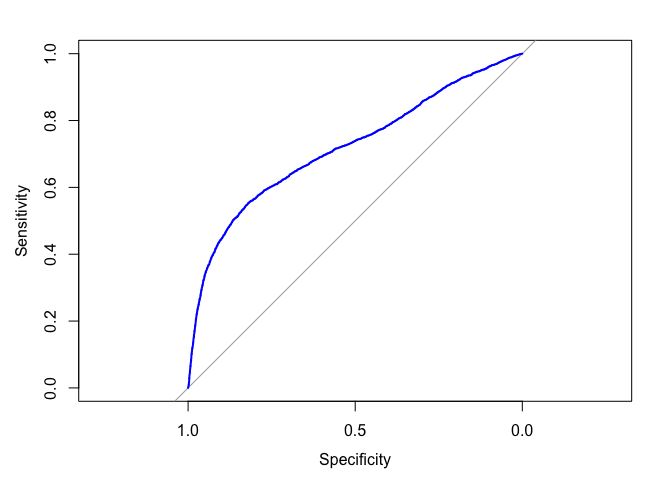
\includegraphics{Modeling-CLV_R-Markdown_files/figure-latex/unnamed-chunk-28-1.pdf}

\begin{Shaded}
\begin{Highlighting}[]
\NormalTok{pROC}\OperatorTok{::}\KeywordTok{auc}\NormalTok{(ROC)}
\end{Highlighting}
\end{Shaded}

\begin{verbatim}
## Area under the curve: 0.7181
\end{verbatim}

\end{document}
